\documentclass{ximera}

\begin{document}
	\author{Stitz-Zeager}
	\xmtitle{TITLE}


\label{ExercisesforAppDerivatives}


In Exercises \ref{incdecderivativeexercisefirst} - \ref{incdecderivativeexerciselast},  use the given function $f$ and its (first) derivative $f'$ to help you find:

\begin{itemize}

\item the open intervals over which $f$ is increasing, decreasing, and constant.

\item the local extrema.

\end{itemize}

Check your answers using a graphing utility.

\begin{enumerate}

\item\label{incdecderivativeexercisefirst} $f(x) = 2x^{3}-3x^{2}-12x + 1$, $f'(x) = 6x^2-6x-12$ % $f''(x) = 12x - 6$

\smallskip

\item $f(x) = \dfrac{10x}{x^2+1}$, $f'(x) = \dfrac{10-10x^2}{\left(x^2+1\right)^2}$ % $f''(x) = \dfrac{20x^3-60x}{\left(x^2+1\right)^3}$

\smallskip

\item\label{incdecderivativeexerciselast} $f(x) = x \sqrt[3]{x-2}$, $f'(x)=\dfrac{4x-6}{3(x-2)^{\frac{2}{3}}}$ % $f''(x)=\frac{4(x-3)}{9(x-2)^{\frac{5}{3}}}$

\smallskip

\setcounter{HW}{\value{enumi}}
\end{enumerate}

In Exercises \ref{concavederivativeexercisefirst} - \ref{concavederivativeexerciselast},  use the given function $f$ and its second derivative $f''$ to help you find:

\begin{itemize}

\item  the open intervals over which the graph of $f$ is concave up and concave down.

\item  the inflection points in the graph.

\end{itemize}

Check your answers using a graphing utility.

\begin{enumerate}
\setcounter{enumi}{\value{HW}}


\item\label{concavederivativeexercisefirst}  $f(x) = 2x^{3}-3x^{2}-12x + 1$,  $f''(x) = 12x - 6$

\smallskip

\item $f(x) = \dfrac{10x}{x^2+1}$,  $f''(x) = \dfrac{20x^3-60x}{\left(x^2+1\right)^3}$

\smallskip

\item\label{concavederivativeexerciselast} $f(x) = x \sqrt[3]{x-2}$, $f''(x)=\dfrac{4(x-3)}{9(x-2)^{\frac{5}{3}}}$ 

\smallskip

\setcounter{HW}{\value{enumi}}
\end{enumerate}

\begin{enumerate}
\setcounter{enumi}{\value{HW}}

\item If $a \neq 0$, we showed in Exercise \ref{quadraticderivativeformulaexercise} in Section \ref{IntroductiontoDerivatives} that if $f(x) = ax^2 + bx + c$, then $f'(x) = 2ax + b$. Solving $f'(x) = 0$ produced $x = -\frac{b}{2a}$, the $x$-coordinate of the vertex of the parabola $y = f(x)$. This Exercise shows this is part of a pattern.

\begin{enumerate}  \item  If $a \neq 0$, show the $x$-coordinate of the $x$-intercept of the graph of $y = ax + b$ is $x = -\frac{b}{a} = -\frac{b}{1 \, a}$.

\item  If $a \neq 0$, for $f(x) = ax^3 + bx^2 + cx + d$ it turns out that $f''(x) = 6ax + 2b$.  Show $x = -\frac{b}{3a}$ is the $x$-coordinate of the inflection point of the graph of $y = f(x)$.

\end{enumerate}

\item\label{MinimizeAverageCostProofExercise}  In Exercise \ref{AverageCostMarginalCostExercise} in Section \ref{FunctionArithmetic}, we observed that average cost appeared to be minimized when average cost was approximately equal to marginal cost.  In this Exercise, we use Calculus and the tools from this section to show this. 

\smallskip

 Recall if $C(x)$ is the cost to produce $x$ items, the \index{average cost}\index{cost ! average}\textbf{average cost} is defined as $\overline{C}(x) = \frac{C(x)}{x}$, $x > 0$,  is the cost per item. 
\begin{enumerate}

\item\label{avgcostcostderivequal}  It turns out that $\overline{C}'(x) = \dfrac{x \, C'(x) - C(x)}{x^2}$.  Show  $\overline{C}'(x) = 0$ when $C'(x) = \overline{C}(x)$.

\smallskip

\item  It turns out that $\overline{C}''(x) = \dfrac{x^2 \, C''(x) - 2x\, C'(x) + 2C(x)}{x^3}$. 

\smallskip

Show we can rewrite this as: $\overline{C}''(x) = \dfrac{x \, C''(x) - 2\, C'(x) + 2 \overline{C}(x)}{x^2}$.

\smallskip

\item\label{reduceavgcostseconderiv}  Show that when $C'(x) = \overline{C}(x)$, then $\overline{C}''(x)  = \frac{C''(x)}{x}$.

\smallskip

\item  It is usually assumed in most economic settings that for cost functions,\footnote{Can you think of reasons why?} $C''(x) > 0$.   Use this and your results from parts \ref{avgcostcostderivequal} and \ref{reduceavgcostseconderiv} to prove that a minimum is produced  when $C'(x) = \overline{C}(x)$.  

\smallskip

\textbf{NOTE:} In Exercise \ref{MarginalCostDerivativeExercise} in Section \ref{IntroductiontoDerivatives}, we saw how $C'(x)$ can be used to approximate the marginal cost, $MC(x)$, so we have established that in order to minimize average cost, we should look where the average cost matches the marginal cost.


\end{enumerate}

\item  The complete graph of $y = f(x)$ is shown below. Use the graph to answer the following questions.

\smallskip


\textbf{NOTE:} Assume $(2.029, 1.82)$ is a local maximum and that $(1.077, 0.948)$ is an inflection point.


\smallskip

\centerline{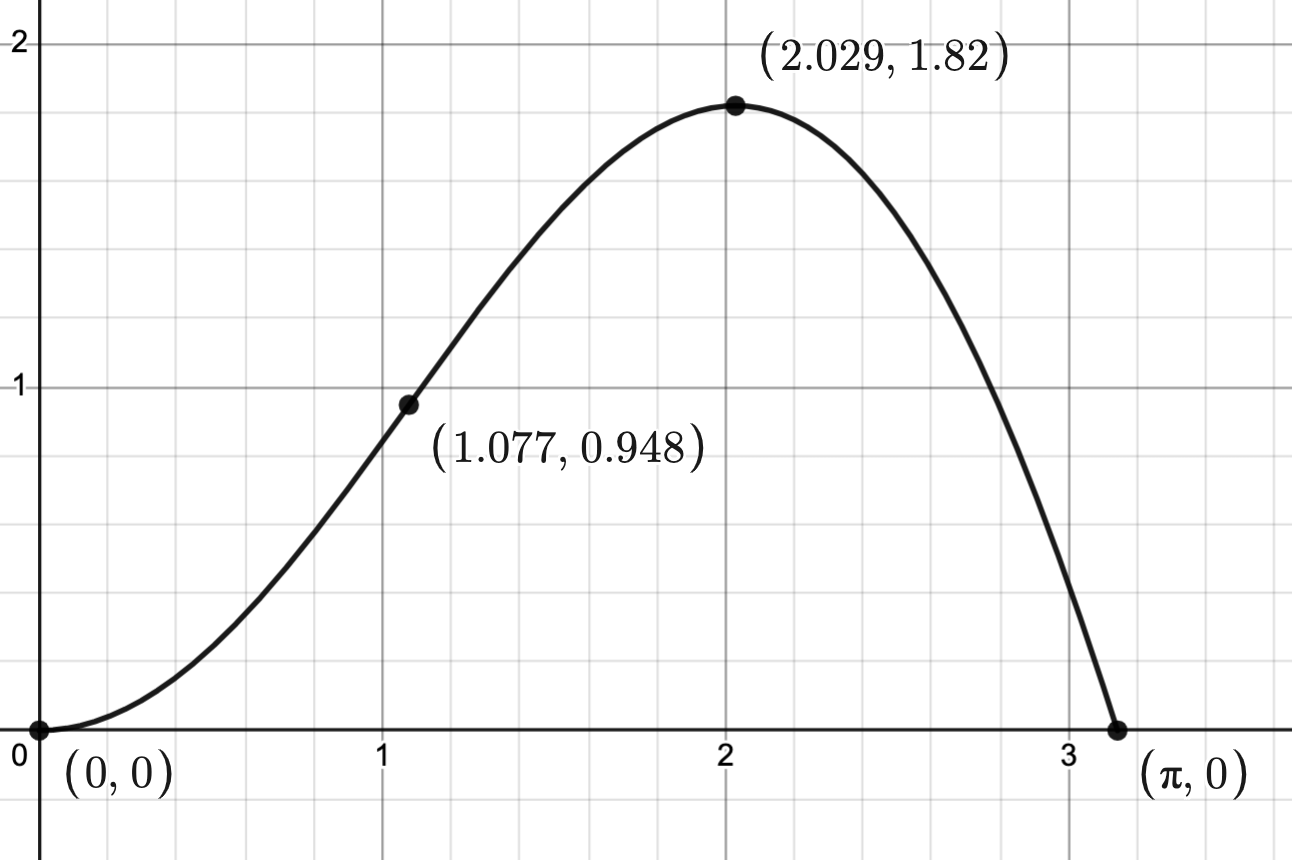
\includegraphics[width = 5in]{./AppDerivativesGraphics/T04Graph.PNG}}

\smallskip

\begin{enumerate}

\item  Determine the $x$-values where:

\begin{multicols}{2}

 $f(x) = 0$:
 
  $f'(x) = 0$:

\end{multicols}

\smallskip

\item List the open intervals over which:

\begin{multicols}{2}

 $f(x) > 0$:
 
  $f(x) < 0$:

\end{multicols}

\smallskip

\begin{multicols}{2}

 $f'(x) > 0$:
 
  $f'(x) < 0$:

\end{multicols}

\smallskip

\begin{multicols}{2}

 $f''(x) > 0$:
 
  $f''(x) < 0$:

\end{multicols}

\end{enumerate}


\item  Below is the graph of $y = f'(x)$ for a \textbf{continuous} function $f$.  

\smallskip

Using Example \ref{graphfromderivativegraphex} as a guide,  sketch a probable graph of $y = f(x)$.  

\begin{center}

\centerline{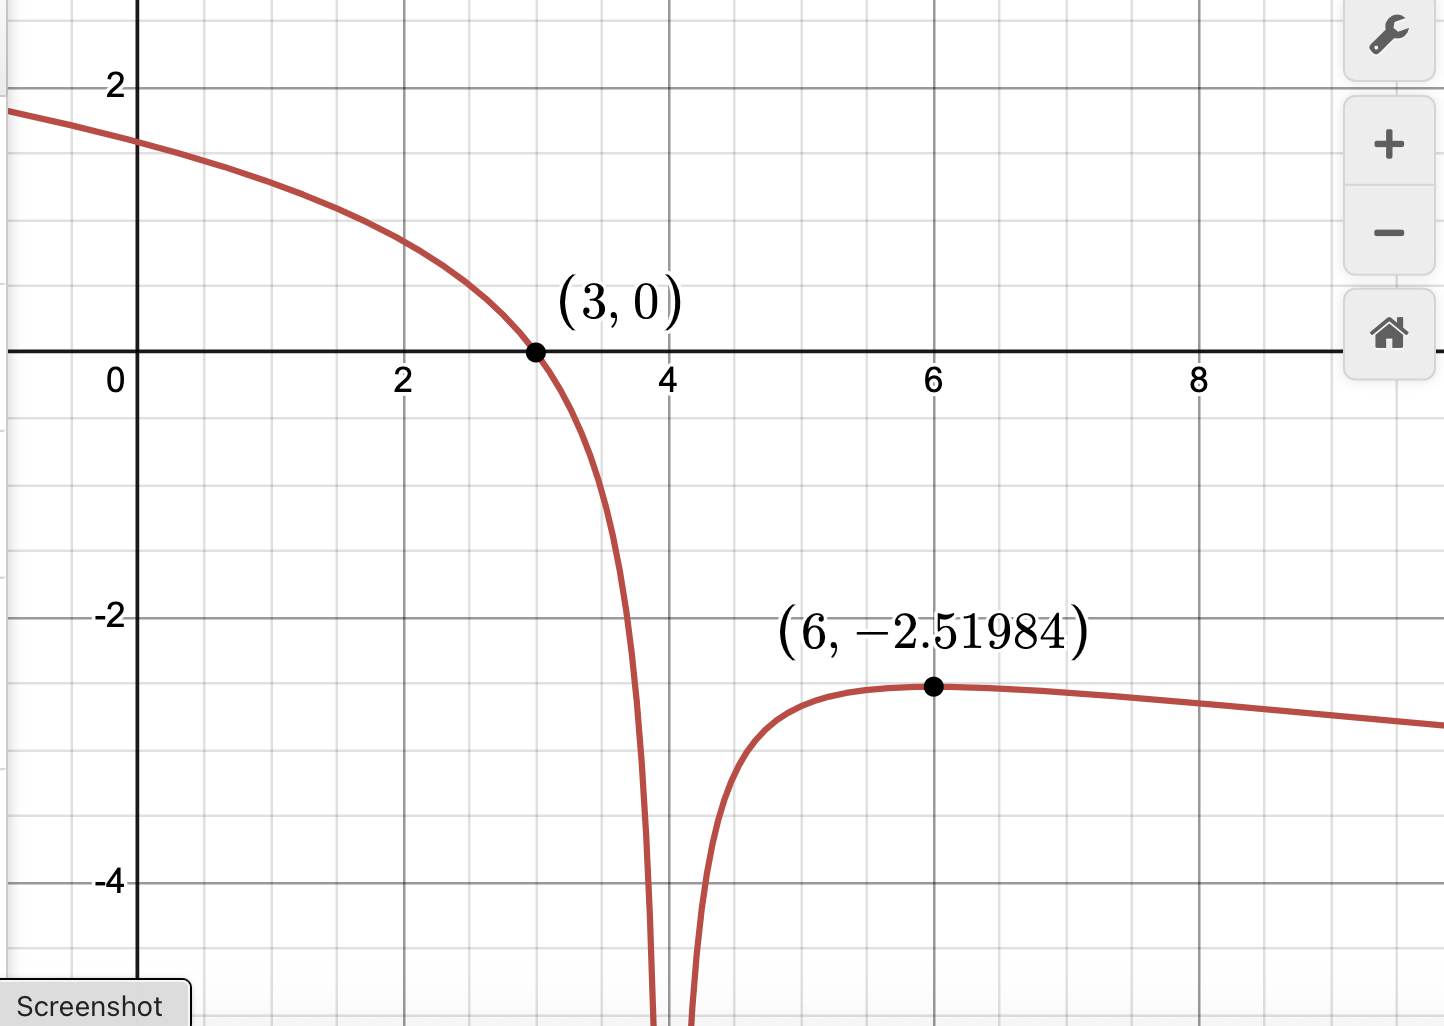
\includegraphics[width = 5in]{./AppDerivativesGraphics/graphfromderivativeexercise.png}}
\end{center}


\newpage

\item  The graph below was taken from https://ohiohospitals.org/covid19data on January 28th, 2021:

\bigskip

\centerline{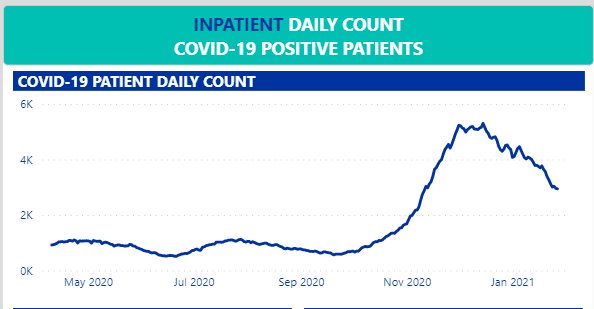
\includegraphics[width = 5in]{./AppDerivativesGraphics/COVIDPatients.PNG}}

\bigskip


With help from your classmate, highlight and label one segment on the graph which (roughly) represents the following scenarios.

\smallskip

For brevity, we'll use `patients' to mean `inpatient COVID positive patients' and `the rate of change' to mean `the rate of change of inpatient COVID positive patients with respect to time.'

\smallskip

\begin{enumerate}

\item  The number of patients is \textbf{decreasing}  \underline{and}  the rate of change is \textbf{decreasing}.  (Label this `a.')

\smallskip

\item  The number of patients is \textbf{decreasing}  \underline{and}  the rate of change  is \textbf{increasing}.  (Label this `b.')

\smallskip


\item  The number of patients is \textbf{increasing}  \underline{and}  the rate of change  is \textbf{increasing}.  (Label this `c.')

\smallskip


\item  The number of patients is \textbf{increasing}  \underline{and}  the rate of change is \textbf{decreasing}.  (Label this `d.')

\smallskip

\item  Discuss with your classmates what the phrase  `flatten the curve' could mean in terms of first and second derivatives.  (See below for an illustration.)


\smallskip

\centerline{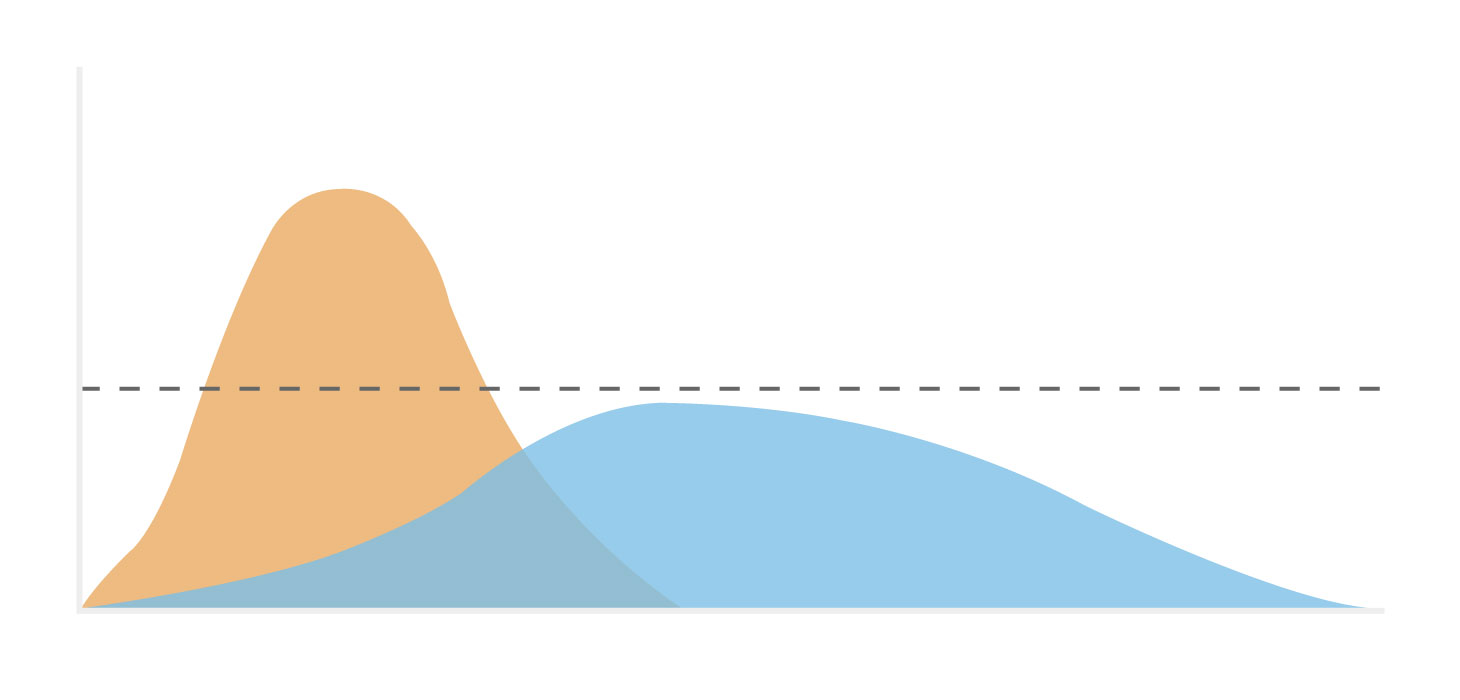
\includegraphics[width = 4.5in]{./AppDerivativesGraphics/flattenthecurve.jpeg}}


\end{enumerate}




\setcounter{HW}{\value{enumi}}
\end{enumerate}

\newpage

\subsection{Answers}

\begin{enumerate}

\item increasing:  $(-\infty, -1)$, $(2, \infty)$;  decreasing:  $(-1,2)$;  local max:  $(-1,8)$;  local min:  $(2, -19)$.

\smallskip

\item increasing:  $(-1,1)$;  decreasing:  $(-\infty, -1)$, $(1, \infty)$;  local max:  $(1,5)$;  local min:  $(-1, -5)$.

\smallskip

\item increasing:  $\left( \frac{3}{2}, \infty\right)$; decreasing:  $\left( -\infty, \frac{3}{2}\right)$;  local (absolute) min:  $\left(\frac{3}{2}, -\frac{3}{2 \sqrt[3]{2}}\right)$

\smallskip

\setcounter{HW}{\value{enumi}}
\end{enumerate}

\begin{enumerate}
\setcounter{enumi}{\value{HW}}


\item  concave up: $\left(\frac{1}{2}, \infty\right)$;  concave down: $\left( - \infty, \frac{1}{2} \right)$; inflection point:  $\left(\frac{1}{2}, \frac{11}{2}\right)$

\smallskip

\item concave up:  $\left( -\sqrt{3}, 0 \right)$, $\left( \sqrt{3}, \infty \right)$;  concave down:    $\left(- \infty,  -\sqrt{3} \right)$, $\left(0,  \sqrt{3} \right)$;  inflection points:  $\left( -\sqrt{3}, -\frac{5 \sqrt{3}}{2} \right)$, $(0,0)$, $\left( \sqrt{3}, \frac{5 \sqrt{3}}{2} \right)$
\smallskip

\item  concave up:  $(-\infty, 2)$, $(3, \infty)$;  concave down:  $(2,3)$;  inflection points: $(2,0)$, $(3, 3)$. 

\smallskip

\setcounter{HW}{\value{enumi}}
\end{enumerate}

\begin{enumerate}
\setcounter{enumi}{\value{HW}}

\item  \begin{enumerate}  \item To find the $x$-intercept, we set $ax+b = 0$  and get $x = -\frac{b}{a}$ provided $a \neq 0$.

\item  Solving  $f''(x) = 6ax + 2b = 0$, we get $x = -\frac{2b}{6a} = - \frac{b}{3a}$, provided $a \neq 0$.  

\smallskip

The graph of $f''(x) =  6ax + 2b$ is a line so we know on one side of $x= - \frac{b}{3a}$, $f''(x) > 0$ and on the other side, $f''(x) < 0$.  

\smallskip

Hence, the graph of the original function $y = f(x)$ changes concavity at $x = -\frac{b}{3a}$.

\end{enumerate}

\item\begin{enumerate}  \item  To solve $\overline{C}'(x) = \dfrac{x \, C'(x) - C(x)}{x^2} = 0$, we set the numerator,  $x \, C'(x) - C(x) = 0$. We get  $x \, C'(x)  = C(x)$ so $C'(x) = \frac{C(x)}{x} = \overline{C}(x)$.

\smallskip

\item  Divide both numerator and denominator of  $\overline{C}''(x) = \dfrac{x^2 \, C''(x) - 2x\, C'(x) + 2C(x)}{x^3}$ by $x$: 

\smallskip

$\overline{C}''(x) = \dfrac{x \, C''(x) - 2 \, C'(x) + 2\frac{C(x)}{x}}{x^2}$ and substitute  $\frac{C(x)}{x} = \overline{C}(x)$.

\smallskip

\item  If  $C'(x) = \overline{C}(x)$, then:

\smallskip

 $\overline{C}''(x)  = \dfrac{x\, C''(x) - 2\, C'(x) + 2\overline{C}(x)}{x^2} =  \dfrac{x\, C''(x) - 2\overline{C} (x) + 2\overline{C}(x)}{x^2}= \dfrac{x\, C''(x)}{x^2} =  \dfrac{C''(x)}{x}$.

\smallskip

\item  When $C'(x) = \overline{C}(x)$, we have that $\overline{C}'(x) = 0$ and $\overline{C}''(x) > 0$.  By the Second Derivative Test for Local Extrema,  Theorem \ref{secondderivatvetest}, the average cost $\overline{C}(x)$ has a minimum when $C'(x) = \overline{C}(x)$ 

\smallskip



\end{enumerate}

\newpage

\item \begin{enumerate}  \item

\begin{multicols}{2}

 $f(x) = 0$:  $x = 0, \pi$
 
  $f'(x) = 0$: $x = 2.029$ ($f_{+}'(0) = 0$.,  too.)

\end{multicols}

\smallskip

\item  \begin{multicols}{2}

 $f(x) > 0$: $(0, \pi)$
 
  $f(x) < 0$: none

\end{multicols}

\smallskip

\begin{multicols}{2}

 $f'(x) > 0$: $(0, 2.029)$
 
  $f'(x) < 0$: $(2.029, \pi)$

\end{multicols}

\smallskip

\begin{multicols}{2}

 $f''(x) > 0$: $(0, 1.077)$
 
  $f''(x) < 0$: $(1.077, \pi)$.

\end{multicols}

\end{enumerate}

\item Answers vary.  below is a sketch of the key features that should be included:


\begin{center}

\centerline{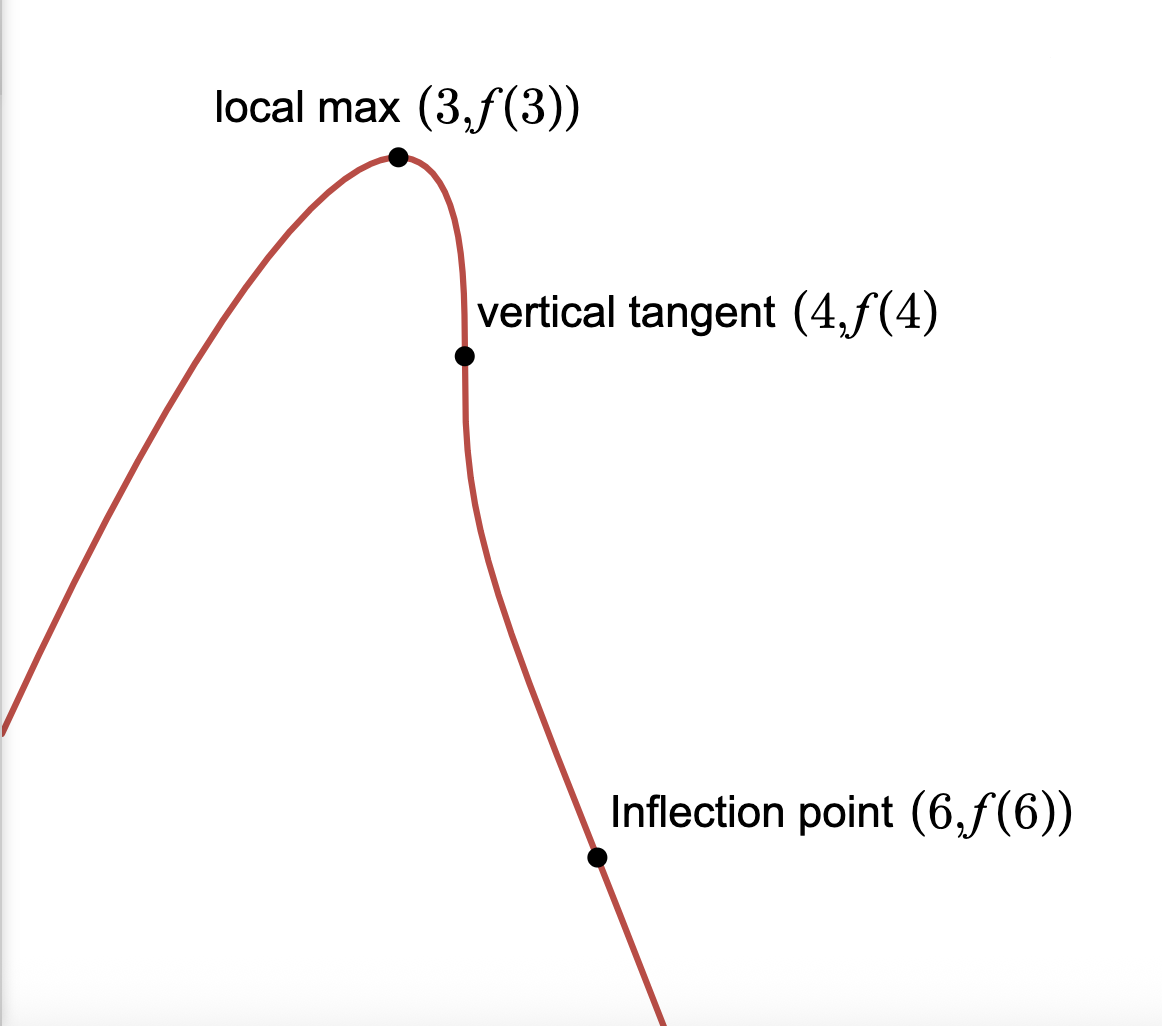
\includegraphics[width = 5in]{./AppDerivativesGraphics/graphfromderivativeexerciseanswer.png}}
\end{center}


\setcounter{HW}{\value{enumi}}
\end{enumerate}




\end{document}
